\chapter{Attack on Prefetcher}

For side-channel attacks to function better and extract data in lesser number
of cycles, they need to isolate the victim to execute memory accesses.
Any other program which may be running will only interfere with the side-channel.
Even if the victim is executing in some other region of code which does not
directly implement the security algorithm, memory accesses of that execution
will also affect the noise in the side channel. Data prefetchers are
also troublesome in this regard because they can generate memory accesses which
did not originate from the victim. This ability is utilised by Disruptive Prefetcher
as seen in \Secref{sec:disruptive-section}.

\section{Motivation}

\begin{figure}[ht]
    \centering
    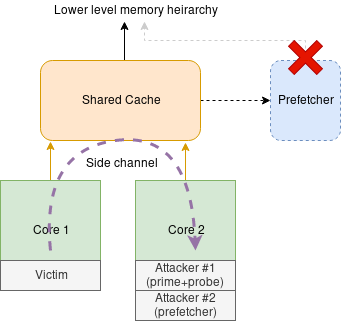
\includegraphics[width=0.6\textwidth]{figures/prefetch_attack}
    \caption{Prevent prefetcher from issuing memory accesses}
    \label{fig:prefetch_attack}
\end{figure}

An attacker with reasonable access to the system which the victim is running on
has the capability to restrict execution of only the victim, along with
isolating the region of code relevant to encryption. But there is no
direct way to restrict the prefetcher from generating memory access.
A separate attack can be mounted on the prefetcher which prevents it
from training on victim addresses and having low confidence to
avoid issuing any prefetches. As seen in \Figref{fig:prefetch_attack}, such an
attacker can run simultaneously with a Prime+Probe attacker.

\section{Implementation}

The most basic form of the prefetcher is a Stride Prefetcher. The PC address,
last memory address and the last stride and confidence counter is
stored in a table and checked whenever there is a cache miss \Citeref{stride_pf}.
If PC address lookup is successful and the stride matches,
the confidence counter is incremented.
If the counter is above a certain threshold, we can say that this stride value
has gained enough confidence to match the program's true patter. This stride
and memory address is used to generate memory accesses separated by the stride
value. For simulation, Stride Prefetcher implementation of gem5 \Citeref{gem5}
has been used which is similar in implementation to what is described here
\Citeref{gem5-stride}.

The victim program may have multiple load instructions which generate a stride
pattern and the PC of these instructions will be recorded by the prefetcher.
The attacker tries to prevent each entry of the prefetcher from training on
any such load instructions of the victim. If there is a chance that the prefetcher
has recorded some load instruction, the attacker tries to evict this entry from
the table by placing its own entry. New entries in the prefetcher are initialised
with a low confidence value by default. If the victim load instruction is eventually
re-entered into the prefetcher table, it will have to retrain to get the confidence
above threshold and this will prevent prefetches from being generated for some time.
The attacker continuously keeps filling the prefetcher with its own entries so that
the victim's entries cannot generate a high enough confidence.

% reduce the
% confidence by giving it a randomly changing stride value and hence keeping
% confidence level low. A low confidence will never lead to the counter
% exceeding threshold to generate prefetches.

To achieve this, the attacker basically has to bombard the prefetcher with
enough load instructions to fill up the whole table.
This is done by placing the instructions at many different PC addresses
which ensure that atleast one load aliases to every entry in the table.
Stride value of access is randomized for every load instruction so that
the prefetcher does not generate prefetches for attacker's loads.
Memory addresses of the load instructions are also restricted to a single cache
line so that the attacker does not interfere with an already running
side-channel attack. This is done by keeping the addresses in same 64-byte boundary.
To ensure there is a cache miss every time, flushing before load using
\texttt{clflush} needs to be done.
If the attacker's loads do not generate a cache miss, prefetcher is never accessed.
\texttt{nop} instructions are used to align loads to the desired PC address.

\subsection{Full attacker}

\Lstref{lst:full_attack} shows a part of the Assembly instructions
which are used in the attacker. These instructions show how loads are
placed at different PC addresses and how they will be able to fill
all entries of the prefetcher. This is called the "full" attacker because
it tries to fill up the whole prefetcher table.

\begin{lstlisting}[caption={Assembly showing load misses at different PCs},
label={lst:full_attack}]
00000000000006ca <attack>:
 6ce:   8b 58 36        mov    0x36(%rax),%ebx
 6d1:   90              nop
 6d2:   0f ae 78 36     clflush 0x36(%rax)
 6d6:   8b 58 08        mov    0x8(%rax),%ebx
 6d9:   90              nop
 6da:   0f ae 78 08     clflush 0x8(%rax)
 6de:   8b 58 3f        mov    0x3f(%rax),%ebx
 6e1:   90              nop
 6e2:   0f ae 78 3f     clflush 0x3f(%rax)
 6e6:   8b 58 38        mov    0x38(%rax),%ebx
 6e9:   90              nop
 6ea:   0f ae 78 38     clflush 0x38(%rax)
 6ee:   8b 58 20        mov    0x20(%rax),%ebx
 6f1:   90              nop
\end{lstlisting}

The drawback of this full attack is that it is extremely slow. There are about
256 loads which all generate a cache miss. The long time which the attacker
takes to execute leads to gaps in the attack. In these gaps, the victim's
load instructions get trained by the
prefetcher and generate memory accesses. To remove the newly trained PC addresses,
the attack loop has to start again which takes a long time.

\subsection{Targeted attacker}

The lesser the loads which we would need to execute, the better this attack will
function. It is possible to conduct offline analysis of victim process
and predict which PC addresses would lead to maximum prefetches being generated.
If these PC addresses are found, only they need to be targeted by the attacker.
Then the number of loads which need to be executed is reduced from ~256 to ~32.
This can be seen in \Lstref{lst:targeted_attack}.

\begin{lstlisting}[caption={Attacker targeting specific PC addresses},
label={lst:targeted_attack}]
00000000000006ca <attack>:
     ...
 6d9:   90                      nop
 6da:   8b 58 0f                mov    0xf(%rax),%ebx
 6dd:   0f ae 78 0f             clflush 0xf(%rax)
 6e1:   90                      nop
 6e2:   90                      nop
 6e3:   90                      nop
 6e4:   8b 58 3c                mov    0x3c(%rax),%ebx
 6e7:   0f ae 78 3c             clflush 0x3c(%rax)
 6eb:   90                      nop
 6ec:   90                      nop
     <nop slide> ...
 6f7:   90                      nop
 6f8:   8b 58 2f                mov    0x2f(%rax),%ebx
 6fb:   0f ae 78 2f             clflush 0x2f(%rax)
 6ff:   90                      nop
     ...
\end{lstlisting}

Only those load instructions which will alias with the victim's loads are
being executed, and the gaps in between are filled with repeating \texttt{nop}
instructions called \texttt{nop} slide. This \texttt{nop} slide will introduce
a very small delay thus reducing the gap which was present in the full attack.

\pagebreak
\section{Simulation and Results}

\subsection{Simulator setup}

\begin{tabular}{|l|r|}
\hline
Simulator  & gem5 X86\\
\hline
Cores#  & 2\\
\hline
L1 Icache & 32K 8-way\\
\hline
L1 Dcache & 32K 8-way\\
\hline
L2 cache & 256K 16-way shared between cores\\
\hline
L2 prefetcher  & Stride 64-entry 4-way, confthresh 4\\
\hline
\end{tabular}
\\

Victim process runs on core1 and attacker runs on core2. Number of prefetches
issued are measured for every 1,000,000 instructions of victim process.

\subsection{Results for benchmarks}

\begin{figure}[h]
    \centering
    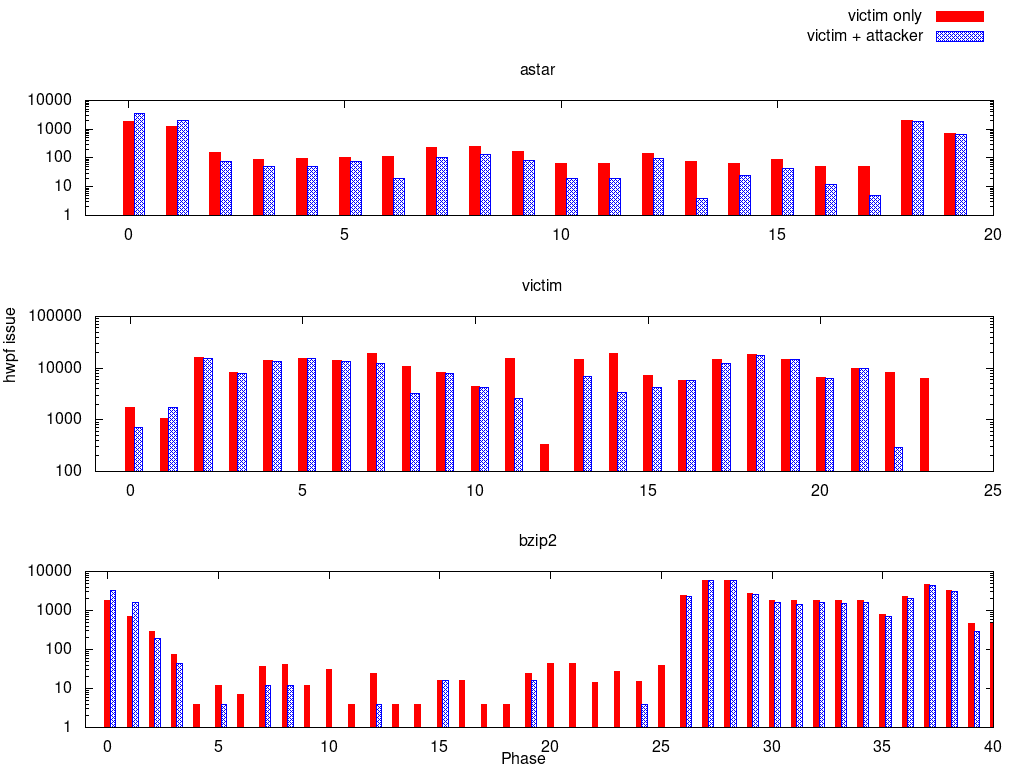
\includegraphics[width=0.95\textwidth]{figures/hwpf_num}
    \caption{Number of prefetches issued on different benchmarks}
    \label{fig:prefetch_attack}
\end{figure}

\begin{figure}[h]
    \centering
    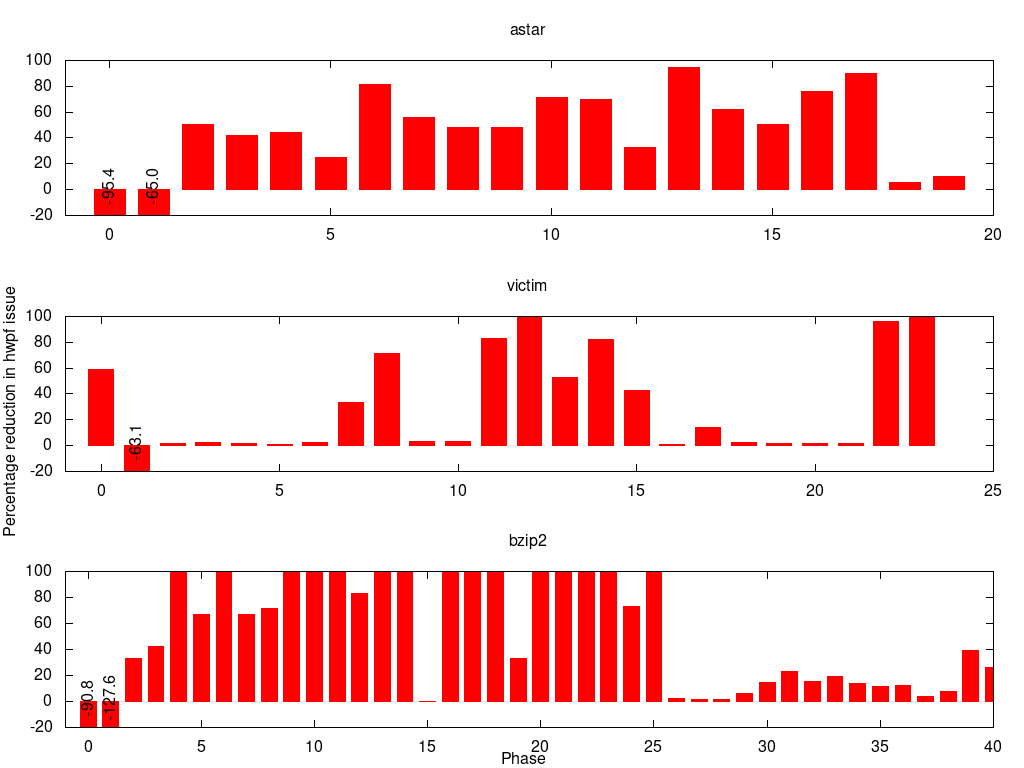
\includegraphics[width=0.95\textwidth]{figures/hwpf_perc}
    \caption{Percentage reduction in number of prefetches}
    \label{fig:prefetch_percred}
\end{figure}

The full attacker implementation is used for \Figref{fig:prefetch_attack} and
\Figref{fig:prefetch_percred}.
These results show the drawback of full attacker where it is not able to
fully eliminate the prefetches issued. This is because of the long execution
time which allows the victim to retrain the prefetcher.

\subsection{Results for AES}

An implementation of AES is best to test for prefetches because that is the code
that will generate memory accesses if any. The following results
in \Figref{fig:targeted_attack} and \Figref{fig:targeted_hitrate} show
number of prefetches and prefetcher table hits vs misses for both
the full attacker and targeted attacker.
As seen in the \Figref{fig:targeted_attack}, a targeted attacker
reduces the number of prefetches issued to zero in most of the phases.
\Figref{fig:targeted_hitrate} shows that this is because more
prefetcher accesses are leading to PC lookup miss than without attacker.
\Figref{fig:targeted_avgconf} also justifies the reduction in prefetches
by full attacker and targeted attacker.
The lower average confidence indicates how well the attack is working.

\begin{figure}[h]
    \centering
    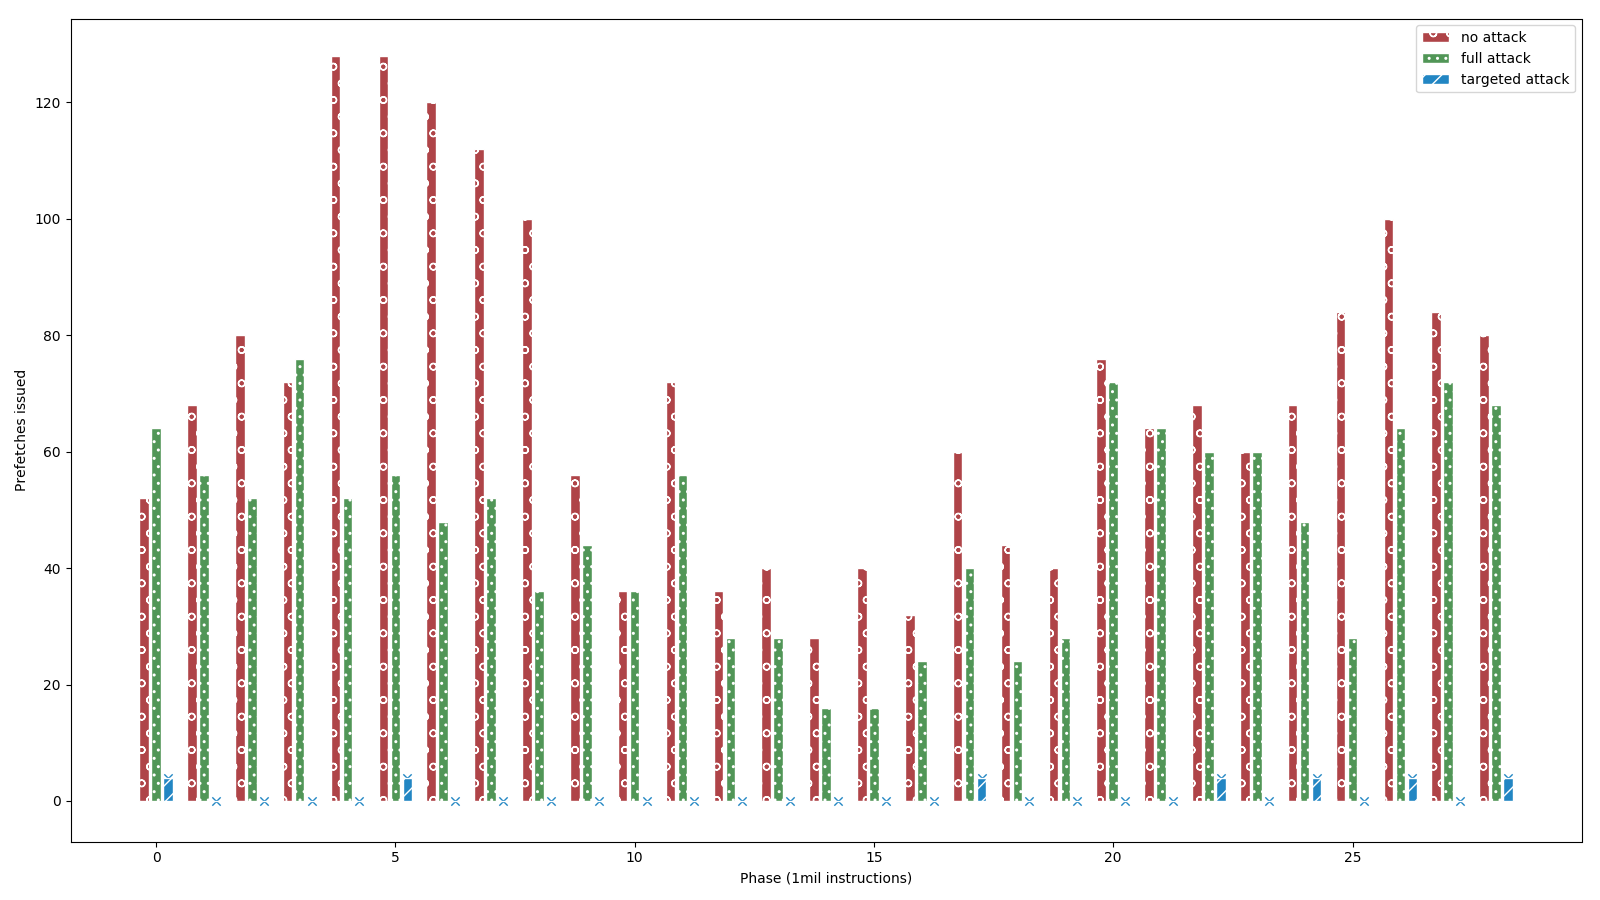
\includegraphics[width=\textwidth]{figures/pf_issued}
    \caption{Comparision of number of prefetches issued by AES program}
    \label{fig:targeted_attack}
\end{figure}

\begin{figure}[h]
    \centering
    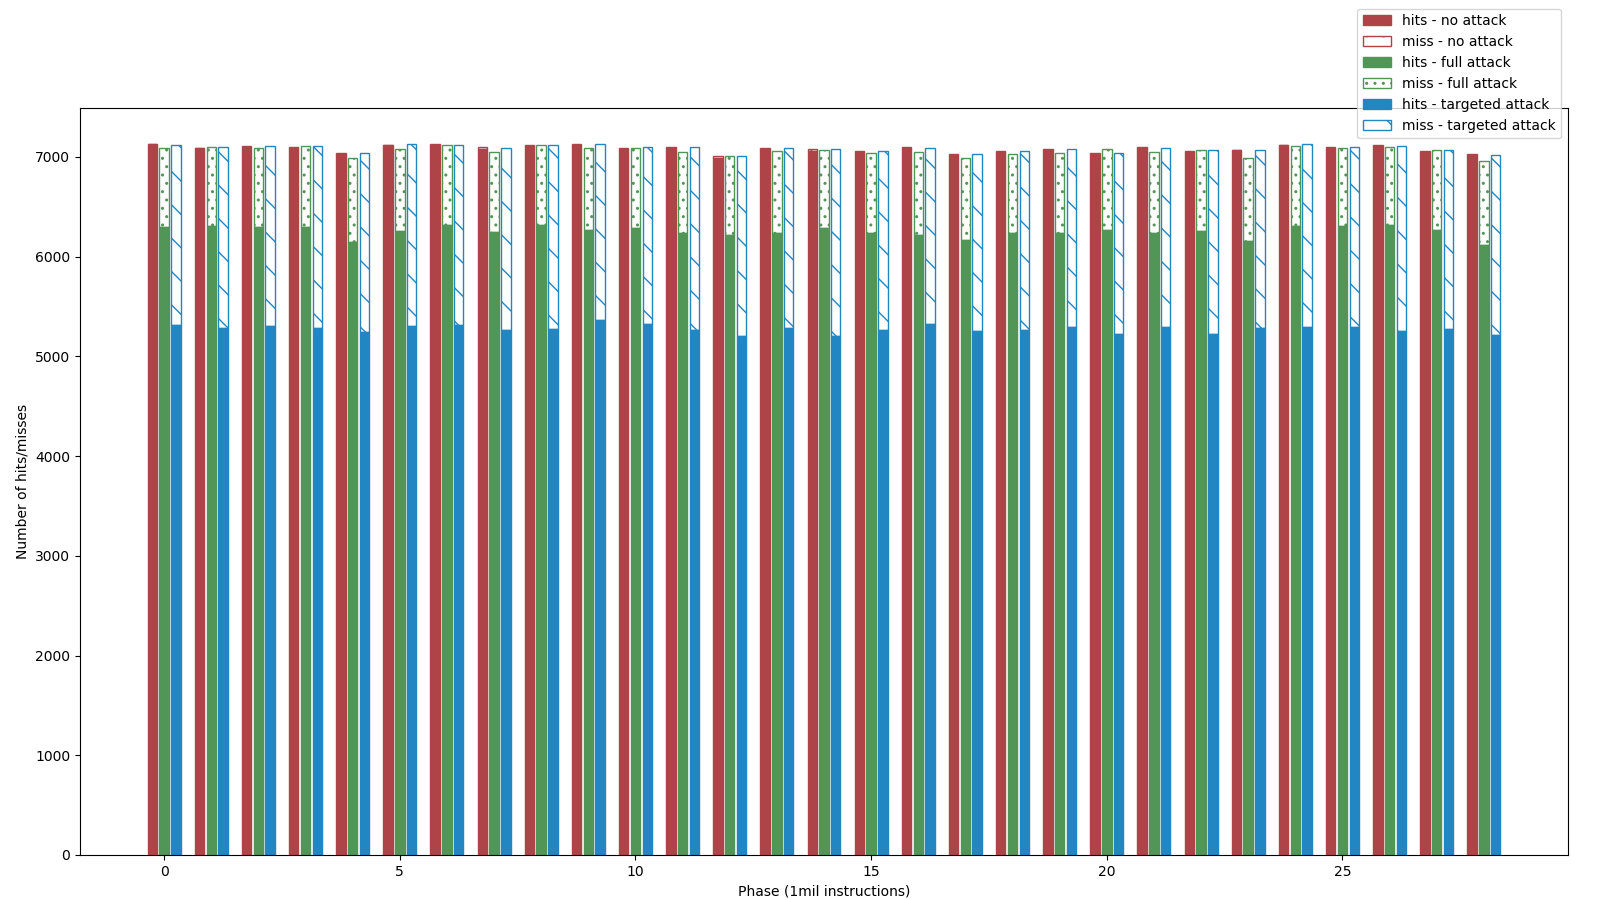
\includegraphics[width=\textwidth]{figures/pf_hits}
    \caption{Comparision of prefetch table hit and miss count by AES program}
    \label{fig:targeted_hitrate}
\end{figure}

\begin{figure}[h]
    \centering
    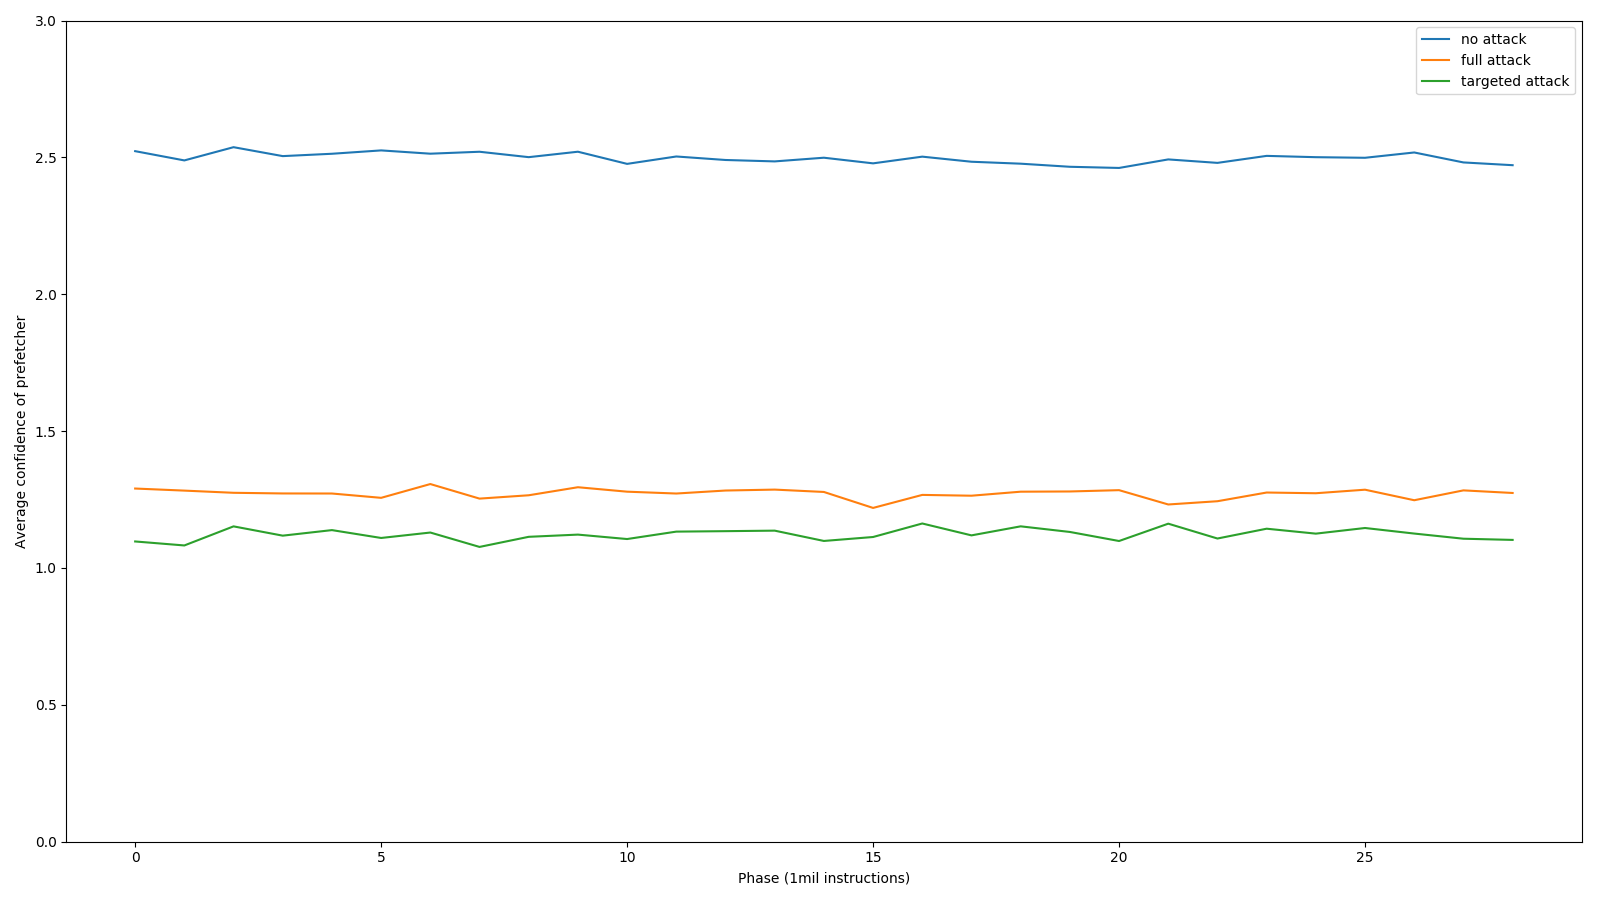
\includegraphics[width=\textwidth]{figures/avg_conf}
    \caption{Comparision of average confidence of prefetcher with AES program}
    \label{fig:targeted_avgconf}
\end{figure}

\subsection{Attack on GHB prefetcher}

Prefetchers can be more efficient if they record more history than
a simple stride. For this purpose, a Global History Buffer is used which
records the data addresses of all load misses in the cache.
An index table stores the PC of load address and a pointer to the GHB
entry containing the last miss address. This pointer is followed in a link-list
fashion through the GHB to get all the previous miss addresses stored
in the buffer.

The previously described attack is tried on a Delta Correlating Prediction Table
(DCPT) \Citeref{dcpt} based prefetcher implemented in \texttt{gem5} \Citeref{gem5-dcpt}.
The same simulation setup is used including same AES program and attacker, only
the prefetcher is changed from Stride to DCPT.
The DCPT prefetcher stores deltas in separate buffers for every table entry instead
of a common GHB. Table entries are indexed based on PC of the load instruction.

\Figref{fig:targeted_dcpt} indicates that the previous attacker works equally well on
a GHB based prefetcher. It is able to reduce the number of issued prefetches from \~1000
to \~10. The full attacker works slightly better than the targeted attacker because
it fills up all the buffers with unwanted loads. The targeted attacker is tailored to
the Stride prefetcher and hence may be miss out other loads which the DCPT prefetcher
is able to capture.

\begin{figure}[h]
    \centering
    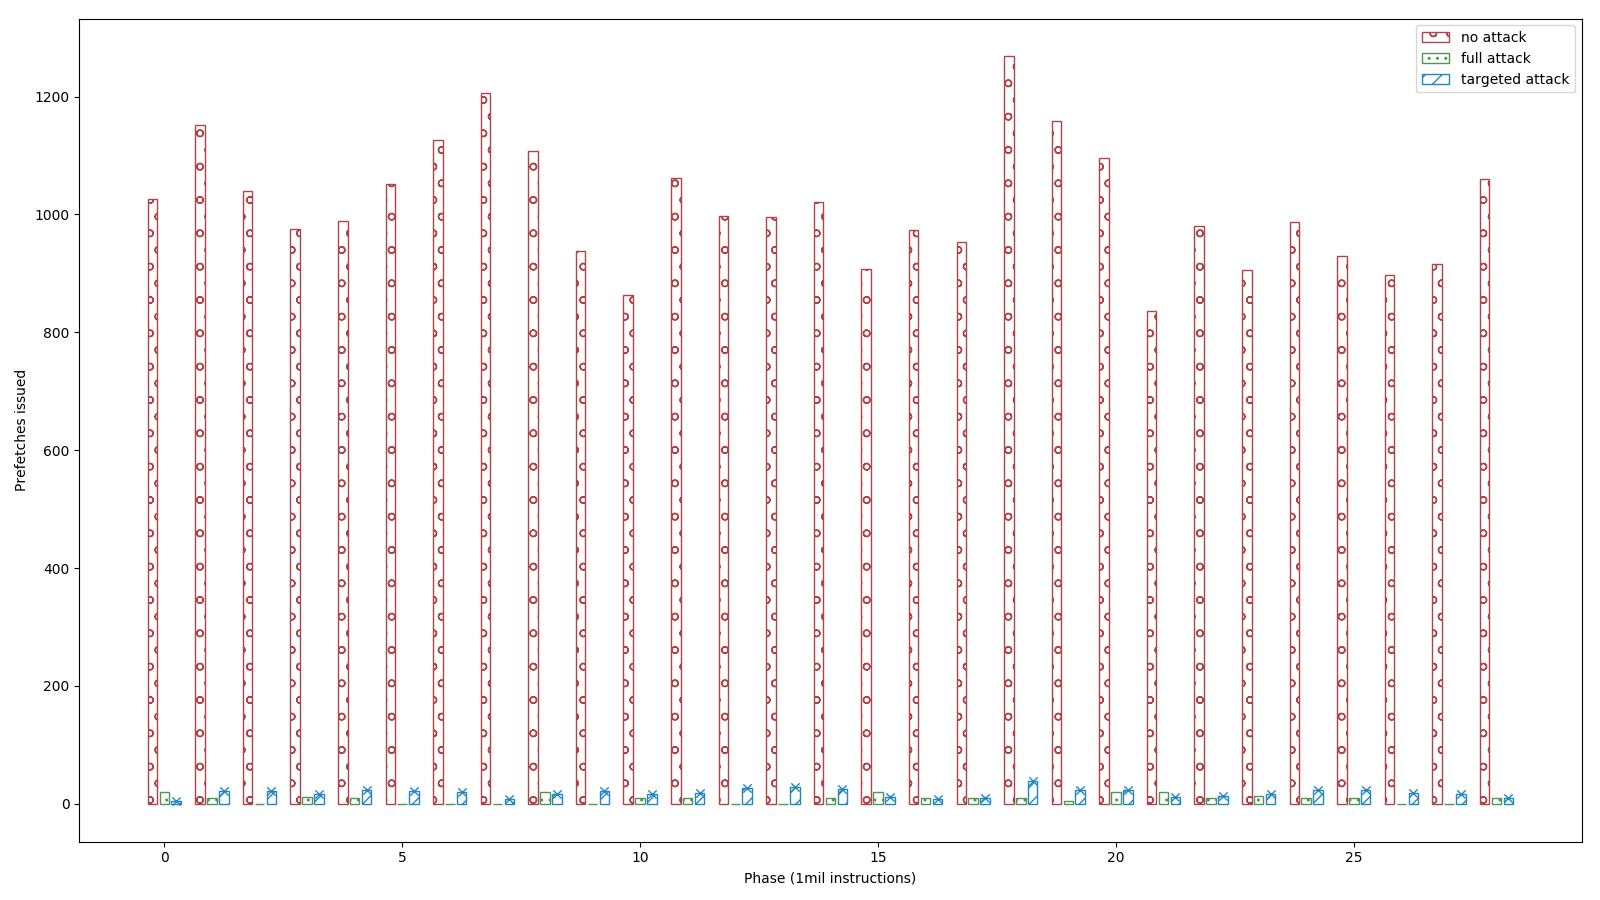
\includegraphics[width=\textwidth]{figures/dcpt-hwpf}
    \caption{Number of prefetches issued by GHB prefetcher}
    \label{fig:targeted_dcpt}
\end{figure}

% I love you meet udeshi. Will you be mine forever and ever and ever? : Yours himani0
